\chapter{Étude de cas - défaillance circuit intégré}
\label{chap:3}
\section{Présentation du produit et de la défaillance}

Dans ce chapitre, une étude de cas de défaillance fonctionnelle d'une fonction de régulation est présentée.
Cette fonction intégrée fait partie d'un produit automobile commercialisé, néanmoins la défaillance est identifiée seulement en réduisant la quantité de composants externes au niveau de la carte.
L'objectif initial était d'étudier l'impact d'une réduction des composants externes sur les performances ESD dans le but de diminuer le coût total du système électronique.
L'architecture de la fonction intégrée est présentée dans un premier temps.
L'environnement et les tests ESD effectués seront ensuite détaillés.
Enfin, la faute sera analysée au regard des résultats obtenus avec les tests.

% Principe de la fonction
La fonction de régulation est chargée principalement de convertir la tension batterie en une alimentation régulée 2.5 V.
Cette alimentation 2.5V est utilisée par d'autres parties du circuit, notamment afin d'alimenter le cœur logique et des fonctions analogiques basse-tension.
La fonction de régulation est découpée en plusieurs sous-fonctions, ou blocs, et son architecture est donnée Fig. \ref{fig:monitored_function}).
Le pré-régulateur limite la tension d'entrée V\textsubscript{batt} pouvant atteindre jusqu'à 40 V, et fournit le signal V\textsubscript{clamp9}.
V\textsubscript{clamp9} alimente les blocs internes à faible consommation, tandis que V\textsubscript{pwr} fournit un plus large courant sous 12 V.
Ensuite, une référence bandgap génère, après un délai de démarrage, une référence à 1.0 V appelée V\textsubscript{ref1p0}.
Ce bandgap fournit aussi une référence de courant à 10\textMu{}A sur I\textsubscript{ref10u}, ainsi qu'un drapeau V\textsubscript{bgok} pour signaler si il est en fonctionnement nominal ou non.
Le régulateur 2.5V génère l'alimentation stabilisée 2.5 V sur V\textsubscript{2p5} à partir de l'entrée non-régulée de puissance V\textsubscript{pwr}, la référence du bandgap ainsi que divers autres signaux auxiliaires.
Il fournit un courant maximal de 20 mA.
L'entrée V\textsubscript{batt} ainsi que la sortie V\textsubscript{2p5} sont toutes deux des broches externes.
La première est connectée à la batterie, et protégée par du filtrage externe dont le but est justement d'être réduit pour diminuer le cout.
La seconde broche a besoin d'une capacité de stabilisation d'au moins 100 nF, qui est trop important pour être intégrée sur silicium et doit donc être connectée en externe.

\begin{figure}[!h]
  \centering
  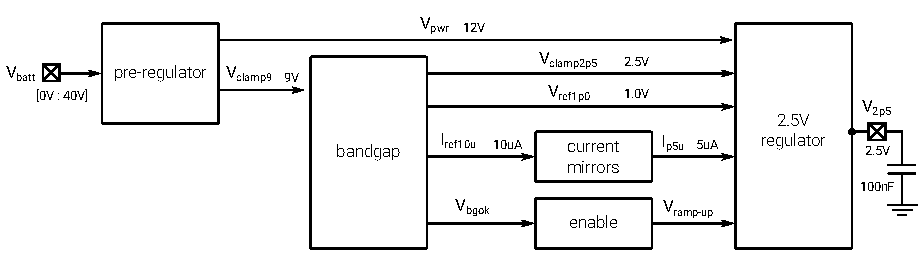
\includegraphics[width=0.9\textwidth]{src/1/figures/monitored_function.pdf}
  \caption{Architecture du primaire d'alimentation}
  \label{fig:monitored_function}
\end{figure}

Cette fonction de régulation fait partie d'un circuit intégré, lui-même faisant partie d'une carte électronique fournissant les divers composants externes requis pour le fonctionnement normal.
L'architecture du système complet est donné Fig. \ref{fig:system_architecture}.
Une campagne de test ESD est effectuée sur cette carte, dans le but d'étudier et de prédire les pertes de fonctionnalités causées par des décharges électrostatiques.
Durant les test, l'ESD est injectée sur la tension batterie en utilisant un motif d'injection DPI \cite{iec62132-4} présenté dans la bibliographie.
Le réseau de filtrage complet comprend une CMC (Common-Mode Choke), un réseau de filtrage LC en Pi ainsi que des capacités des découplages.
La CMC et le filtre en Pi sont enlevés avant les tests afin de tester la configuration réduite.

\begin{figure}[!h]
  \centering
  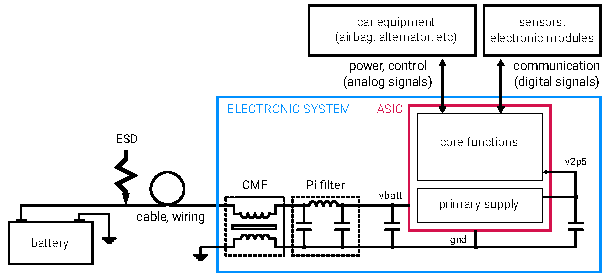
\includegraphics[width=0.9\textwidth]{src/1/figures/architecture_system.pdf}
  \caption{Vue d'ensemble de l'architecture du système}
  \label{fig:system_architecture}
\end{figure}


% Principe défaillance
La défaillance de ce système est observée sur V\textsubscript{2p5}.
Elle est induite en injectant une forte impulsion transitoire d'amplitude négative sur V\textsubscript{batt}, lorsque le produit est alimenté et en fonctionnement normal.
Sur la sortie V\textsubscript{2p5}, la défaillance prends la forme d'une très courte perturbation, suivie d'un arrêt long de la régulation puis de son redémarrage (Fig. \ref{fig:meas-reset-v2p5}).
La durée de la défaillance est d'approximativement 40 \textmu{}s, depuis la perturbation initiale jusqu'au redémarrage.
Elle est bien plus longue que la perturbation d'entrée sur V\textsubscript{batt} (100 ns), ce qui semble indiquer une large faute fonctionnelle dans le circuit.

\begin{figure}[!h]
  \centering
  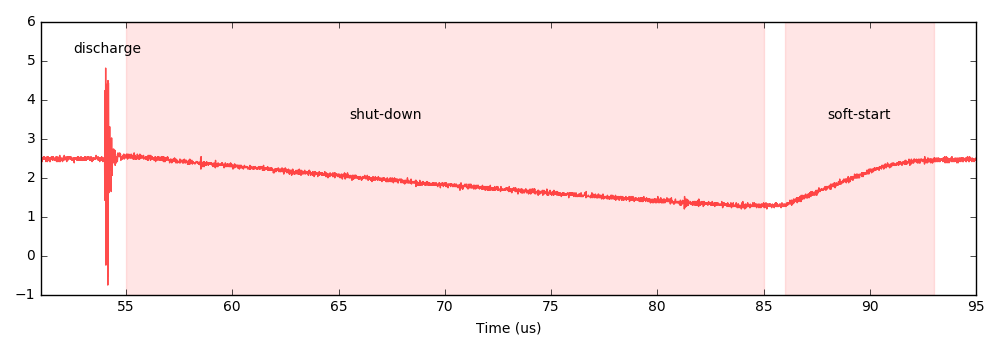
\includegraphics[width=0.9\textwidth]{src/1/figures/v2p5_measure.png}
  \caption{Mesure de V\textsubscript{2p5} après une stress rectangulaire -450 V 100 ns}
  \label{fig:meas-reset-v2p5}
\end{figure}

% What is the root cause -> reset of regulator, soft-start
Il semble donc que le stress négatif injecté sur V\textsubscript{batt} déclenche une séquence de redémarrage, alors que le régulateur est déjà démarré.
Ces séquences de démarrage sont longues car les tensions d'alimentations sont montées doucement afin de protéger l'électronique sensible connectée en aval.
Si un ESD déclenche une telle séquence, le système se retrouve indisponible pendant un délai important.
L'architecture de la fonction intégrée a été présentée précédemment, et est composée de plusieurs blocs.
La question qui se pose à ce stade est de déterminer lequel ou lesquels de ces blocs est responsable de la défaillance.
Deux approches sont possibles, soit par des mesures, soit avec les outils de simulation.
Les simulations sont un outil très intéressant et pratique, mais elles n'ont à ce jour pas été utilisées dans la littérature pour étudier des défaillances fonctionnelles au niveau circuit-intégré.
Il est donc nécessaire d'obtenir des mesures pour évaluer leur fiabilité dans un contexte ESD.

La première partie du travail est focalisée sur le développement de méthodes de mesures directement sur silicium, de façon à comprendre les mécanismes mis en jeu dans l'apparition de la faute.
L'objectif est d'acquérir des données fiables directement au niveau circuit, ce qui est difficile à faire de manière externe.
Ces mesures ont aussi pour objectif de valider les simulations pour l'investigation.
Un véhicule de test a été développé, contenant différentes méthodes de mesure et d'observation.

\section{Présentation du véhicule de test}

% Architecture
L'architecture du véhicule de test est donnée Fig. \ref{architecture_testchip}.
Il contient deux instances de la même fonction de régulation.
La première instance est la fonction sous-test, exposée à des décharges électrostatiques pendant la campagne de tests et dont le comportement est surveillé afin de détecter les fautes.
Cette première instance est placée en configuration réduite sans la plupart des éléments de filtrage externes.
La seconde instance alimente les systèmes de surveillance qui sont intégrés sur puce.
Elle est placée en configuration blindée, avec le réseau de filtrage complet ainsi que des capacités de découplage supplémentaires.
Ces mesures la protègent normalement face à tout résidu ESD pouvant l'atteindre pendant les tests.
Les systèmes de surveillance contiennent notamment des détecteurs de surtension et sous-tension.
Il y a au total 35 détecteurs de ce type dans la puce.
Leurs rôles individuels sont donnés dans le document final.
Le bus de communication permet de lire les données provenant des capteurs et de les configurer ou les remettre à zéro.

\begin{figure}[h]
  \centering
  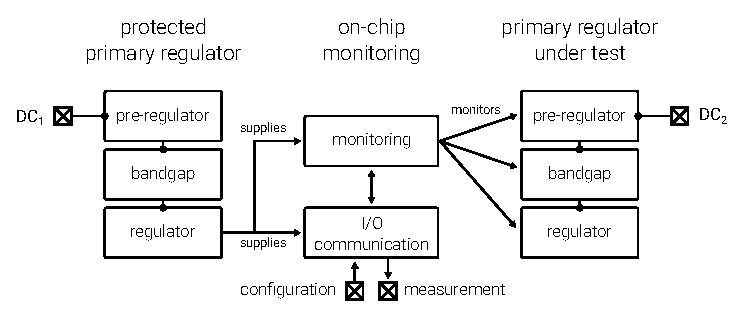
\includegraphics{src/1/figures/architecture_testchip.pdf}
  \caption{Architecture du véhicule de test}
  \label{architecture_testchip}
\end{figure}

Le layout de la puce complète est donné Fig. \ref{fig:top-cell-layout}.
Il est possible d'identifier à droite et à gauche chaque instance de la fonction de régulation.
Les fonctions de régulation ont volontairement été placées de part et d'autre de la puce afin d'éviter des problèmes de couplages d'ESD pendant les tests, qui auraient pu perturber l'alimentation de référence.
Les systèmes de surveillance sont localisés en dessous de ces deux blocs.
Des capteurs de courant sur puce sont localisés à plusieurs endroit contre l'anneau de métal \textit{gndsub} entourant toute la puce.
Beaucoup d'espace a été laissé libre sur le layout, pour des contraintes de fabrication.

\begin{figure}[!h]
  \centering
  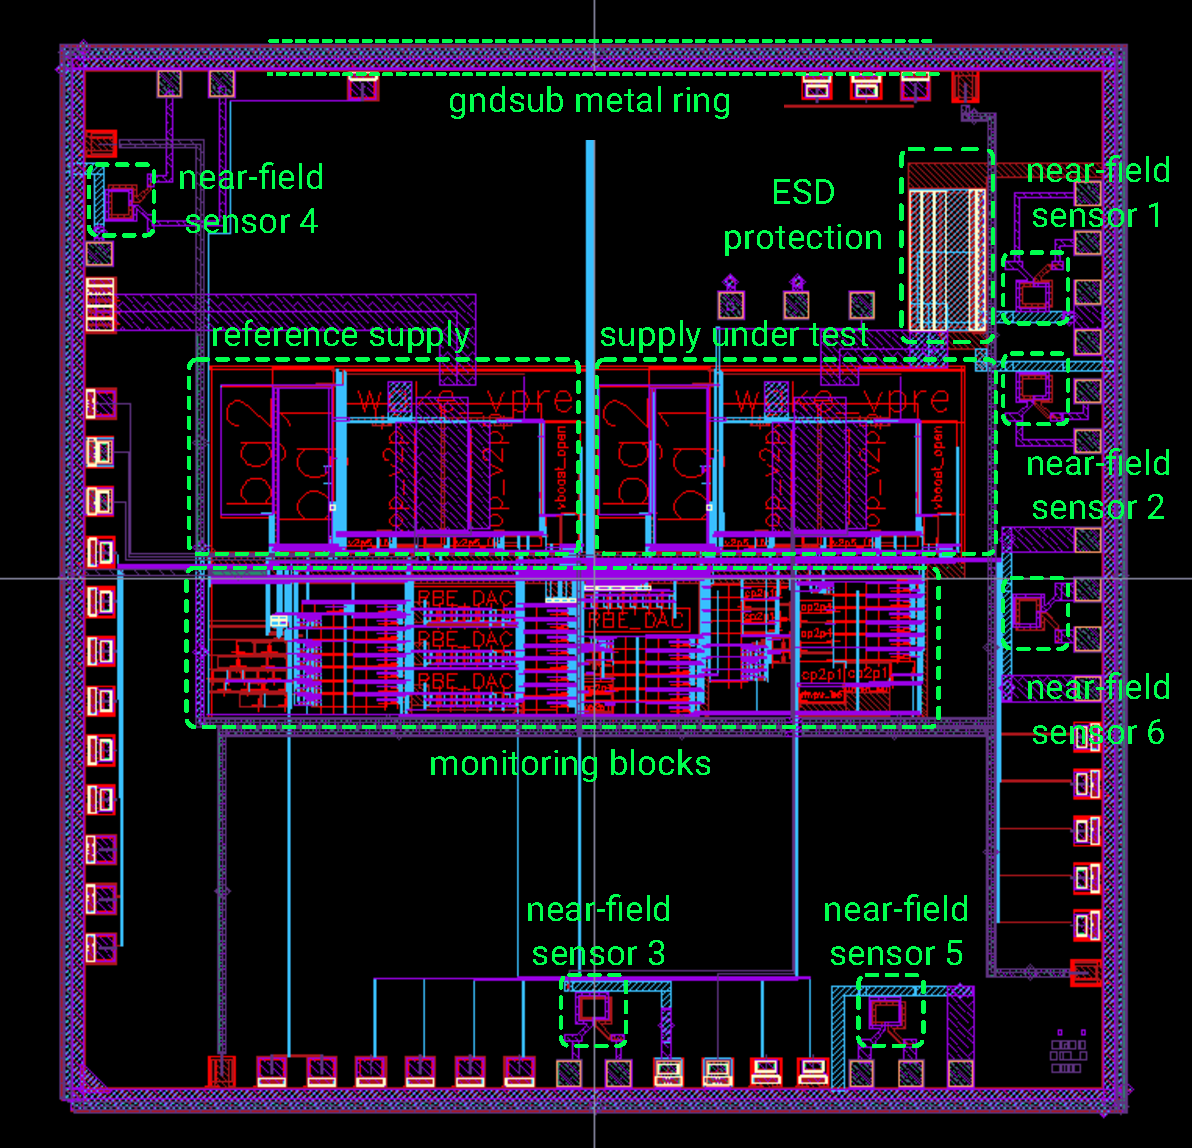
\includegraphics[width=0.7\textwidth]{src/1/figures/topcell_layout.pdf}
  \caption{Layout de la top-cell}
  \label{fig:top-cell-layout}
\end{figure}

% What is a current sensors
Dans le véhicule de test, on trouve également des capteurs de courant directement intégrés sur silicium, qui permettent de mesurer un courant circulant dans une piste placée à proximité.
Par couplage, le capteur génère une tension proportionnelle à la dérivée du courant dans la piste.
La figure \ref{fig:near-field-current-sensor} donne une représentation 3D du capteur.
Ce type de boucle de courant intégré sur silicium a été originellement désigné et étudié par A. Salles dans \cite{OtherInductors, InductorsLAAS1, InductorsLAAS2, AlainSallesInductors}.

\begin{figure}[!h]
  \centering
  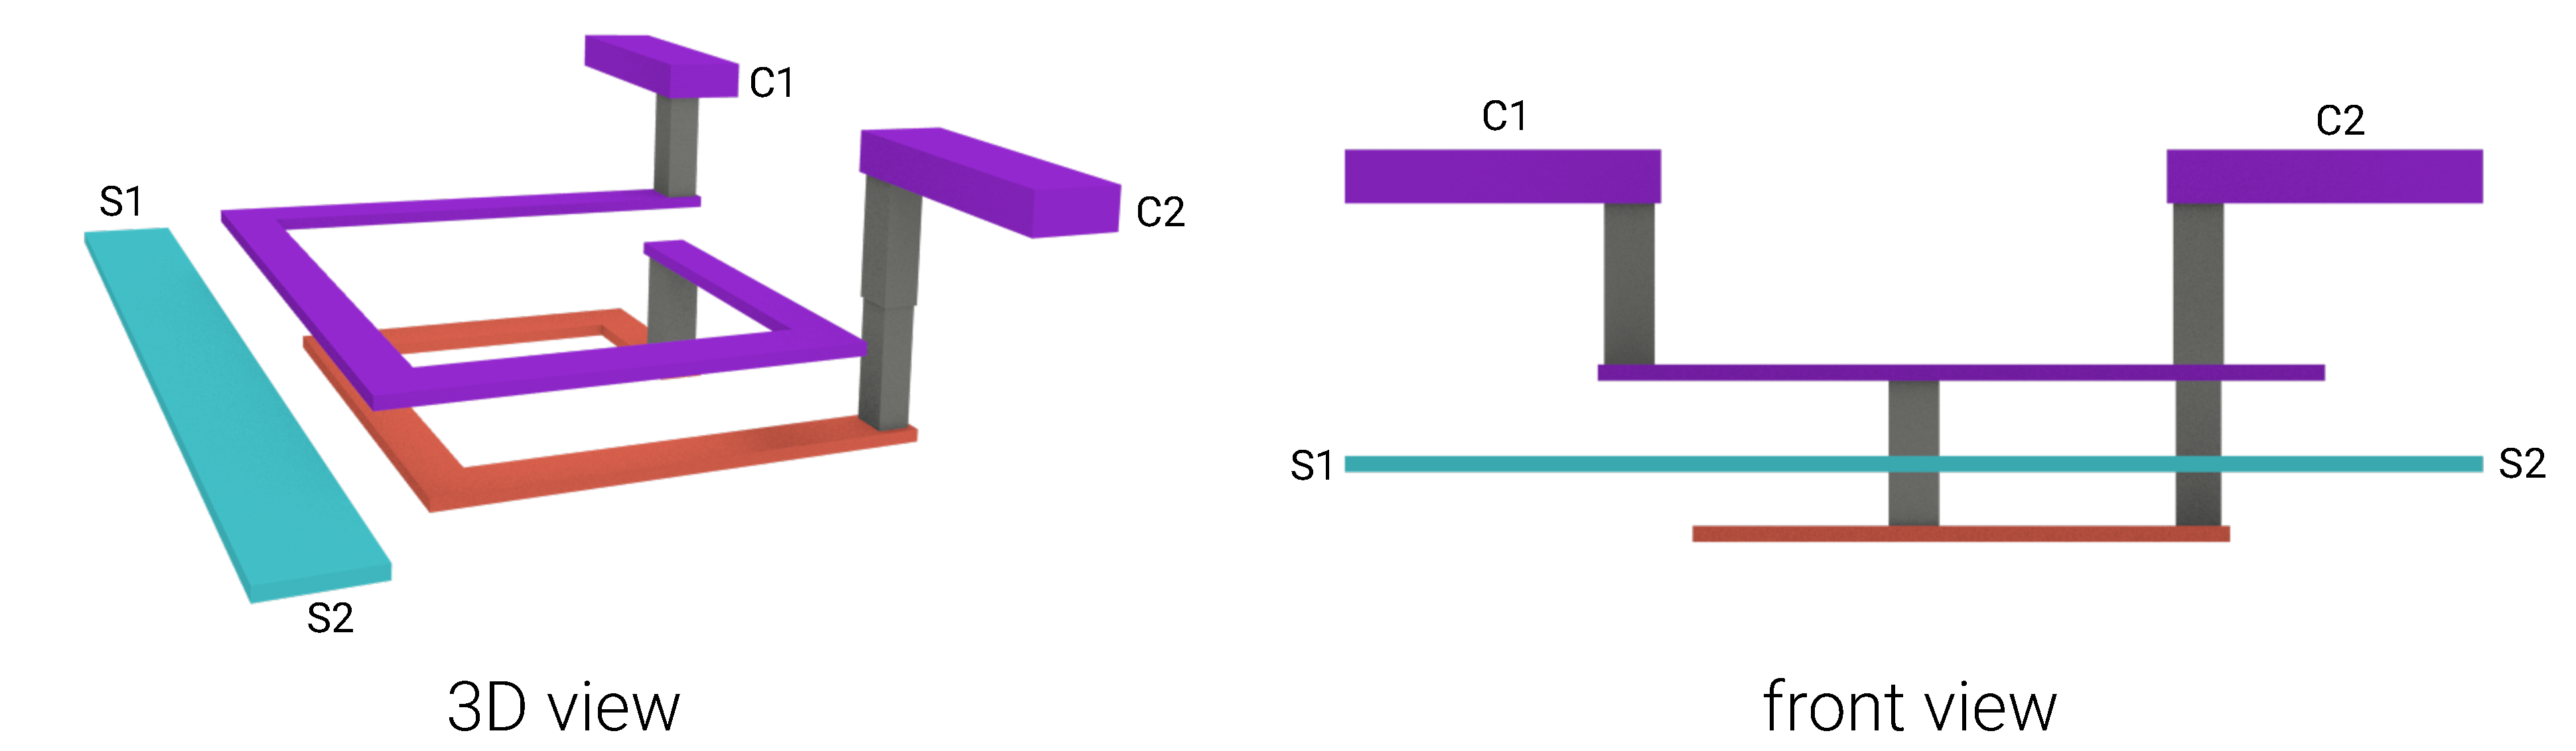
\includegraphics[width=0.98\textwidth]{src/1/figures/near-field-current-sensor.pdf}
  \caption{Design du capteur de champ-proche}
  \label{fig:near-field-current-sensor}
\end{figure}

% How is it designed and how is it used
Sur silicium, trois niveaux de métaux sont requis pour construire ce capteur.
Le premier niveau en rouge (Fig \ref{fig:near-field-current-sensor}) et le troisième niveau en violet forment une boucle métallique.
Des vias connectent les différents niveaux ensembles.
La piste mesurée est elle localisée au deuxième niveau.
Le courant mesuré circule entre les nœuds \textit{S1} et \textit{S2}.
Un oscilloscope avec une impédance d'entrée 50 \textOmega{} est utilisé pour mesurer la tension différentielle entre \textit{C1} et \textit{C2}.

% Talk about the near-field current sensors placement
Au total, 6 capteurs de courant sont implémentés sur la puce.
Un des capteurs est dédié à la calibration.
Les autres capteurs mesurent des courant sur des points importants du circuits, là où des résidus de décharges ESD sont susceptibles de se propager.
Le capteur \textit{1} mesure le courant sur l'entrée batterie.
Le capteur \textit{2} mesure le courant absorbé par la protection ESD protégeant l'entrée batterie.
Le capteur \textit{3} mesure le courant à travers la capacité externe de stabilisation du régulateur.
Enfin, les capteurs \textit{4} et \textit{5} mesurent les courants évacués les deux connexions externes à la masse via l'anneau métallique \textit{gndsub}.

\subsection{Résultats}

Une fois la puce de test fabriquée et assemblée dans un package, des tests préliminaires ont été conduits afin de la valider.
Les alimentations intégrées sur silicium sont toutes deux pleinement fonctionnelles et fournissent des alimentations à 2.5V valides.
Dans le cas de l'alimentation de référence, cela signifie que les blocs de surveillance ont été correctement dimensionnés pour le courant maximum que peut délivrer l'alimentation.

Par contre, des problèmes ont été rencontrés avec le bus de communication.
De multiples essais on étés effectués, mais il est toujours impossible d'obtenir une réponse fiable du bus.
Il fut suspecté dans un premier temps que l'impact d'éléments parasites au niveau silicium l'empêchait de fonctionner correctement.
Néanmoins, des simulations \textit{back-annotées} contenant la netlist des blocs ainsi que des éléments parasites extraits du layout n'ont pas permis de reproduire le produire sur l'ensemble des simulations de vérifications.
Un problème de délai fut aussi suspecté, mais également impossible à reproduire même en plaçant des délais importants à tous les endroits possibles.
Finalement, des problèmes de couplage substrats pourraient expliquer le comportement erratique, mais les fréquences de fonctionnement basses du bus semblent exclurent ce type de perturbation.
Des investigations futures pourront être conduites afin de déterminer le problème et de le corriger, car le concept de ce bus de communication pouvant être facilement implémenté sur une schématique reste intéressant pour des véhicules de tests.

Le bilan est plus positif pour les capteurs de courants.
Ils sont opérationnels et permettent de mesurer le courant avec un bonne sensibilité.
Le capteur connecté en amont de la protection ESD protégeant l'entrée batterie à survécu à des décharges appliquées directement sur cette entrée.
Les mesures obtenues par ces capteurs sont exploitées afin de valider les simulations de courant entrant et sortant de la puce, ainsi que de la répartition du courant propagé dans la puce.
